\documentclass[a3paper,12pt]{article}
\title{\heiti 物理海洋学笔记}
\author{\small 2017级海洋科学专业 崔英哲 \\ \small \url{https://github.com/Cuiyingzhe/Physical-Oceanography-Notes/}}
\date{\small 2020.07.06}
\usepackage[UTF8]{ctex}
%\usepackage{indentfirst}
\usepackage{geometry}
\usepackage{amsmath}
\usepackage{booktabs}
\usepackage{tabu}
\usepackage{caption}
%\usepackage{gensymb}
\usepackage{graphicx}
\usepackage{float}
\usepackage{cite}
\usepackage{hyperref}
\usepackage{cases}
\usepackage{esint}
\usepackage{fancyhdr}
\usepackage{CJK}
\usepackage{titlesec}
\usepackage{titletoc}
\usepackage{mathrsfs}
\usepackage{harpoon}
\usepackage{amssymb}
\usepackage{color}
\usepackage{bm}
\usepackage{framed}
\usepackage{setspace}
%\usepackage[T1]{fontenc}
%\usepackage{mathptmx}
\hypersetup{
	colorlinks=true,
	linkcolor=black,
	citecolor=blue
}
\captionsetup[table]{labelsep=space,font={small}}
\captionsetup[figure]{labelsep=space,font={small}}
\geometry{a3paper,left=4cm,right=4cm,top=4cm,bottom=4cm}
\graphicspath{{C:/Users/Gary/Desktop/物理海洋学/note}}
\begin{document}
    \maketitle
    \renewcommand*\contentsname{}
	\tableofcontents
    \newpage
    \section{基本方程}
    \subsection{旋转坐标系的速度和加速度}
    \setlength{\parindent}{0pt}
    惯性坐标系:
    静止的或是匀速直线运动的坐标系,固定在恒星上的坐标系可以被看成惯性坐标系.\\
    固定在地球上的坐标系:
    地球对恒星的加速度主要是由地球自转引起的,于是可以把地球当作一个对惯性坐标系作纯粹地转运动的物体.
    \subsubsection{旋转坐标系和惯性坐标系中的速度}
    \begin{figure}[H]
		\centering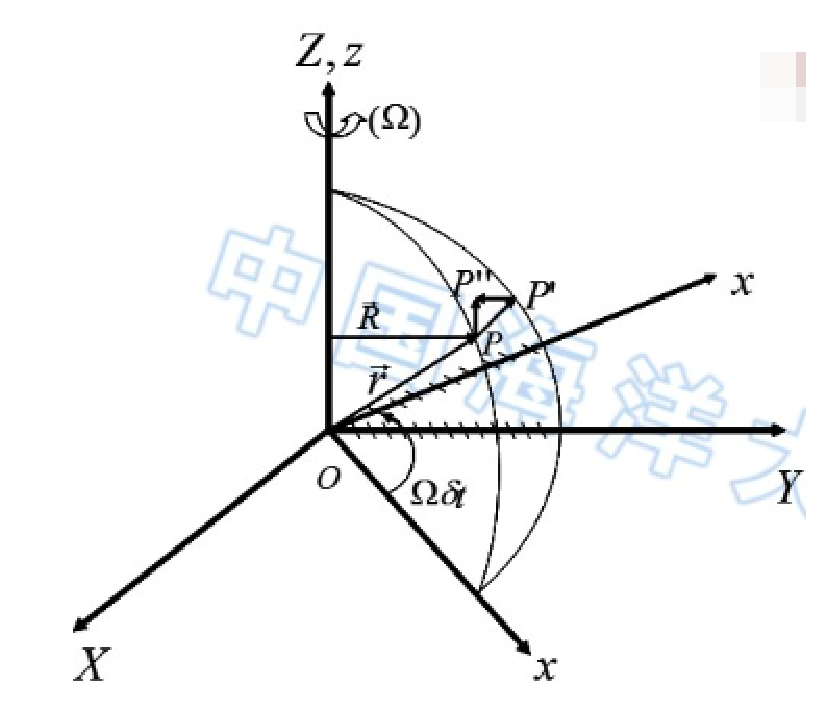
\includegraphics[width=7cm]{1.eps}
		\caption*{}
    \end{figure}
    惯性坐标系($XYZ$)绝对位移:$\vec{pp''}=\vec{V}_a\delta t, \vec{V}_a$为绝对速度\\
    旋转坐标系($xyz$)相对位移:$\vec{p'p''}=\vec{V}\delta t, \vec{V}$为相对速度\\
    $\because \vec{pp''}=\vec{p'p''}+\vec{pp'}$ \\
    $\therefore\vec{V}_a\delta t=\vec{V}\delta t+\vec{V}_e\delta t\Rightarrow\vec{V}_a=\vec{V}+\vec{V}_e$(绝对速度等于相对速度与牵连速度的向量和)\\
    其中,$\vec{V}_e=\vec{\Omega}\times\vec{r}\Rightarrow\vec{V}_a=\vec{V}+\vec{\Omega}\times\vec{r}$
    \[
        \Rightarrow\frac{d_a\vec{r}}{dt}=\frac{d\vec{r}}{dt}+\vec{\Omega}\times\vec{r}
    \]
    \[
        \frac{d_a\vec{A}}{dt}=\frac{d\vec{A}}{dt}+\vec{\Omega}\times\vec{A}
    \]
    \subsubsection{旋转坐标系和惯性坐标系中的加速度}
    令$\vec{A}=\vec{V}_a=\vec{V}_e+\vec{V}=\vec{V}+\vec{\Omega}\times\vec{r}$
    \begin{equation*}
        \begin{aligned} \frac{d \bar{V}_{a}}{d t} &=\frac{d_{a}}{d t}\left(\vec{V}+\vec{V}_{e}\right)=\frac{d_{a}}{d t}(\vec{V}+\vec{\Omega} \times \vec{r}) \\ &=\frac{d}{d t}(\vec{V}+\vec{\Omega} \times \vec{r})+\vec{\Omega} \times(\vec{V}+\vec{\Omega} \times \vec{r}) \\ &=\frac{d \vec{V}}{d t}+\vec{\Omega} \times \vec{V}+\vec{\Omega} \times \vec{V}+\vec{\Omega} \times(\vec{\Omega} \times \vec{r}) \\ &=\frac{d \vec{V}}{d t}+2 \vec{\Omega} \times \vec{V}-\Omega^{2} \vec{R} \end{aligned}
    \end{equation*}
    \subsection{作用在海水微团上的外力 运动方程的向量形式}
    压强梯度力:$\displaystyle\frac{1}{\rho}\nabla p$\\
    分子粘性力(摩擦力):
    \[
        \left\{
        \begin{aligned}
            &F_{x}=\frac{1}{\rho} \mu\left[\frac{\partial^{2} u}{\partial x^{2}}+\frac{\partial^{2} u}{\partial y^{2}}+\frac{\partial^{2} u}{\partial z^{2}}\right]=\frac{\mu}{\rho} \Delta u\\
            &F_{y}=\frac{1}{\rho} \mu\left[\frac{\partial^{2} v}{\partial x^{2}}+\frac{\partial^{2} v}{\partial y^{2}}+\frac{\partial^{2} v}{\partial z^{2}}\right]=\frac{\mu}{\rho} \Delta v\\
            &F_{2}=\frac{1}{\rho} \mu\left[\frac{\partial^{2} w}{\partial x^{2}}+\frac{\partial^{2} w}{\partial y^{2}}+\frac{\partial^{2} w}{\partial z^{2}}\right]=\frac{\mu}{\rho} \Delta w
        \end{aligned}
        \right.
        \Rightarrow \vec{F}=\frac{\mu}{\rho}\Delta \vec{V}=\gamma\Delta\vec{v}
    \]
    重力(地球引力与地球自转产生的惯性离心力的合力):$\displaystyle\vec{g}=-G\frac{M_g}{r^2}\cdot\left(\frac{\vec{r}}{r}\right)$\\
    科氏力:$\displaystyle -2\vec{\Omega}\times\vec{V}$\\
    天体引潮力(受其他天体万有引力与惯性力离心力的合力):$\displaystyle\vec{F_M}=-G\frac{M_M}{L^2}+G\frac{M_M}{D^2}\cdot\left(\frac{\vec{D}}{D}\right)$\\
    由牛顿第二定律和坐标系转换关系:
    \[
        \left\{
        \begin{aligned}
            &\frac{d_{a} \vec{V}_{a}}{d t}=\sum_{i} \vec{F}_{t}\\
            &\frac{d_{a} \vec{A}_{a}}{d t}=\frac{d \vec{V}}{d t}+2 \vec{\Omega} \times \vec{V}-\Omega^{2} \vec{R}
        \end{aligned}
        \right.
    \]
    \[
        \Rightarrow\boxed{\color{red} \frac{d \vec{V}}{d t}=-\frac{1}{\rho} \nabla P-2 \vec{\Omega} \times \vec{V}+\vec{g} +\nu \Delta \vec{V}+\vec{F}_{T}}
    \]
    \subsection{运动方程在球坐标系的标量形式}
    \begin{figure}[H]
        \centering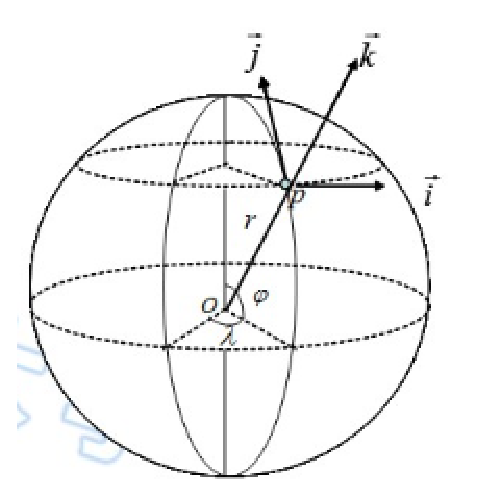
\includegraphics[width=5cm]{2.eps}
        \caption*{}
    \end{figure}
    速度:
    \[
        \vec{V}=u\vec{i}+v\vec{j}+w\vec{k}
    \]
    \[
        \Rightarrow
        \left\{\begin{array}{l}u=r \cos \varphi \frac{d \lambda}{d t} \\ v=r \frac{d \varphi}{d t} \\ w=\frac{d r}{d t}\end{array}\right.
    \]
    加速度:
    \[
        \begin{aligned}
        \frac{d\vec{A}}{dt}&=\frac{\frac{\partial \vec{A}}{\partial t} d t+\frac{\partial \vec{A}}{\partial \lambda} d \lambda+\frac{\partial \vec{A}}{\partial \varphi} d \varphi+\frac{\partial \vec{A}}{\partial r} d r}{dt}\\
        &=\frac{\partial \bar{A}}{\partial t}+\frac{\partial \vec{A}}{\partial \lambda} \frac{d \lambda}{d t}+\frac{\partial \vec{A}}{\partial \varphi} \frac{d \varphi}{d t}+\frac{\partial \vec{A}}{\partial r} \frac{d r}{d t}\\
        &=\frac{\partial \vec{A}}{\partial t}+\frac{u}{r \cos \varphi} \frac{\partial \vec{A}}{\partial \lambda}+\frac{v}{r} \frac{\partial \vec{A}}{\partial \varphi}+w \frac{\partial \vec{A}}{\partial r}
        \end{aligned}
    \]
    \[
        \begin{aligned}
        &\Rightarrow\frac{d}{d t}=\frac{\partial}{\partial t}+u \frac{\partial}{r \cos \varphi \partial \lambda}+v \frac{\partial}{r \partial \varphi}+w \frac{\partial}{\partial r}\\
        &\Rightarrow\boxed{\bm{ \frac{d}{d t}=\frac{\partial}{\partial t}+(\vec{V} \cdot \nabla)}}\\
        &\Rightarrow\boxed{\bm{ \nabla=\frac{\partial}{r \cos \varphi \partial \lambda} \vec{i}+\frac{\partial}{r \partial \varphi} \vec{j}+\frac{\partial}{\partial r} \vec{k}}}
        \end{aligned}
    \]
    \[
        \Rightarrow
        \left\{
            \begin{aligned}
                &\frac{d \vec{i}}{d t}=\frac{\partial \vec{i}}{\partial t}+u \frac{\partial \vec{i}}{r \cos \varphi \partial \lambda}+v \frac{\partial \vec{i}}{r \partial \varphi}+w \frac{\partial \vec{i}}{\partial r}\\
                &\frac{\partial \vec{j}}{d t}=\frac{\partial \vec{j}}{\partial t}+u \frac{\partial \vec{j}}{r \cos \varphi \partial \lambda}+v \frac{\partial \vec{j}}{r \partial \varphi}+w \frac{\partial \vec{j}}{\partial r}\\
                &\frac{d \vec{k}}{d t}=\frac{\partial \vec{k}}{\partial t}+u \frac{\partial \vec{k}}{r \cos \varphi \partial \lambda}+v \frac{\partial \vec{k}}{r \partial \varphi}+w \frac{\partial \vec{k}}{\partial r}
            \end{aligned}
        \right.
    \]
    \newpage
    \[
        \begin{aligned}
            &\frac{d \vec{V}}{d t}=\frac{d u}{d t} \vec{i}+\frac{d v}{d t} \vec{j}+\frac{d v}{d t} \vec{k}+u \frac{d \vec{i}}{d t}+v \frac{d \vec{j}}{d t}+w \frac{d \vec{k}}{d t}\\
            \Rightarrow&\boxed{\color{red}\frac{d \vec{V}}{d t}=\left(\frac{d u}{d t}-\frac{u v t g \varphi}{r}+\frac{u w}{r}\right) \vec{i}+\left(\frac{d v}{d t}+\frac{u^{2} \operatorname{tg} \varphi}{r}+\frac{v w}{r}\right) \vec{j}+\left(\frac{d w}{d t}-\frac{u^{2}+v^{2}}{r}\right)}
        \end{aligned}
    \]
    压强梯度力:
    \[
        \frac{1}{\rho}\nabla p=-\frac{1}{\rho}\left(\frac{1}{r \cos \varphi} \frac{\partial p}{\partial \lambda} \vec{i}+\frac{1}{r} \frac{\partial p}{\partial \varphi} \vec{j}+\frac{\partial p}{\partial r} \vec{k}\right)
    \]
    重力:
    \[
        \vec{g}=-g\vec{k}
    \]
    科氏力:
    \begin{figure}[H]
        \centering 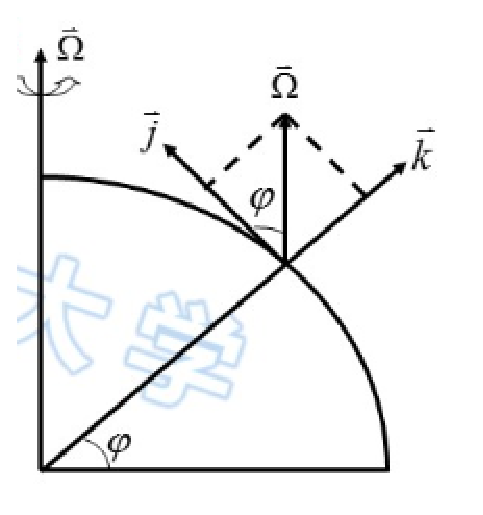
\includegraphics[width=4cm]{3.eps}
        \caption*{}
    \end{figure}
    \vspace{-2cm}
    \[
        \vec{\Omega}=\Omega \sin \varphi \vec{k}+\Omega \cos \varphi \vec{j}
    \]
    \[
        \begin{aligned}
            -2 \vec{\Omega} \times \vec{V}&=-2\left|\begin{array}{ccc}\vec{i} & \vec{j} & \vec{k} \\ 0 & \Omega \cos \varphi & \Omega \sin \varphi \\ u & v & w\end{array}\right|\\
            &=-2[(w \Omega \cos \varphi-v \Omega \sin \varphi) \vec{i}+(u \Omega \sin \varphi) \vec{j}+(-u \Omega \cos \varphi) \vec{k}]
        \end{aligned}
    \]
    \[
        \Rightarrow-2 \vec{\Omega} \times \vec{V}=(f v-\tilde{f} w) \vec{i}-(f u) \vec{j}+(\tilde{f} u) \vec{k}
    \]
    其中,$\displaystyle\left\{\begin{aligned}&f=2\Omega sin\varphi\\ &\tilde{f}=2\Omega cos\varphi\end{aligned}\right.$
    \[
        \Rightarrow
        \boxed{
        \left\{
        \begin{aligned}
            &\frac{d u}{d t}=-\frac{1}{\rho} \frac{\partial p}{r \cos \varphi \partial \lambda}+f v-\tilde{f} w+\frac{u v \tan \varphi}{r}-\frac{u w}{r}+\gamma(\Delta \vec{v})_{\lambda}-\frac{1}{r \cos \varphi} \frac{\partial \phi_{T}}{\partial \lambda}\\
            &\frac{d y}{d t}=7 \frac{1}{\rho} \frac{\partial p}{r \partial \varphi}-f u-\frac{u^{2} \tan \varphi}{r}-\frac{v w}{r}+\gamma(\Delta \bar{v})_{\varphi}-\frac{1}{r} \frac{\partial \phi_{T}}{\partial \varphi}\\
            &\frac{d w}{d t}=-\frac{1}{\rho} \frac{\partial p}{\partial r}+\tilde{f} u=g+\frac{u^{2}+v^{2}}{r}+\gamma(\Delta \vec{v})_{r}-\frac{\partial \phi_{T}}{\partial r}
        \end{aligned}
        \right.
        }
    \]
    \subsection{直角坐标系的运动方程}
    略去地球曲率的影响
    \[
        \Rightarrow
        \boxed{
        \left\{
        \begin{aligned}
            &\frac{d u}{d t}=-\frac{1}{\rho} \frac{\partial p}{\partial x}+f v+\tilde{f} w+F_{N \lambda}+F_{T \lambda}\\
            &\frac{d v}{d t}=-\frac{1}{\rho} \frac{\partial p}{\partial x}-f u+F_{N y}+F_{T y}\\
            &\frac{d w}{d t}=-\frac{1}{\rho} \frac{\partial p}{\partial z}+\tilde{f} u-g+F_{N z}+F_{T z}
        \end{aligned}
        \right.
        }
    \]
    \subsection{海水层流运动的基本方程组}
    \subsubsection{连续方程}
    \[
        \frac{\partial \rho}{\partial t}+\nabla \cdot(\rho \vec{V})=0 \Leftrightarrow \frac{d \rho}{d t}+\rho \nabla \cdot \vec{V}=0
    \]
    特别地,对于不可压缩流体:
    \[
        \nabla \cdot \vec{V}=0
    \]
    \subsubsection{盐量扩散方程}
    \[
        \mathop{\frac{\partial}{\partial t} \iiint\limits_{\tau} \rho s d \tau}\limits^{\mbox{盐量增加量}}=\mathop{-\oiint\limits_{\sigma} \rho s V_{n} d \sigma}\limits^{\mbox{平流作用}}+\mathop{-\oiint\limits_{\sigma} S_{n} d \sigma}\limits^{\mbox{分子扩散作用}}
    \]
    \[
        \begin{aligned}
            &\iiint\limits_{\tau} \frac{\partial (\rho s)}{\partial t} d \tau =\iiint\limits_{\tau} \nabla \cdot(\rho s \vec{V}) d \tau -\iiint\limits_{\tau} \nabla \cdot \vec{S} d \tau \\
            \Rightarrow&\frac{\partial(\rho s)}{\partial t}+\nabla \cdot(\rho s \vec{V})+\nabla \cdot \vec{S}=0\\
            \Rightarrow&\rho \frac{\partial s}{\partial t}+s \frac{\partial \rho}{\partial t}+s \nabla \cdot(\rho \vec{V})+\rho \vec{V} \cdot \nabla s+\nabla \cdot \vec{S}=0\\
            \Rightarrow&\left(\frac{\partial s}{\partial t}+\vec{V} \cdot \nabla s\right)+\frac{s}{\rho}\left[\frac{\partial \rho}{\partial t}+\nabla \cdot(\rho \vec{V})\right]=-\frac{1}{\rho} \nabla \cdot \vec{S}\\
            \Rightarrow&\frac{\partial s}{\partial t}+\vec{V} \cdot \nabla s=\frac{k}{\rho} \Delta s=k_{D} \Delta s
        \end{aligned}
    \]
    其中,$\displaystyle k_{D}=\frac{k}{\rho} \sim 1.1 \times 10^{-9}\left(\mathrm{m}^{2} / \mathrm{s}\right)$
    \subsubsection{热传导方程}
    与上面类似:
    \[
        \frac{\partial \theta}{\partial t}+\vec{V} \cdot \nabla \theta=\frac{\kappa}{\rho c_{p}} \Delta \theta=k_{\theta} \Delta \theta
    \]
    其中,$\displaystyle k_{\theta}=\frac{\kappa}{\rho c_{p}} \sim 1.4 \times 10^{-7}\left(\mathrm{m}^{2} / \mathrm{s}\right)$
    \subsubsection{热膨胀方程-状态方程}
    热膨胀方程:
    \[
        \rho=\mathop{\rho_0}\limits^{\mbox{0℃时的海水密度}}(1-\mathop{k} \limits^{\mbox{海水的热膨胀系数}} \theta)
    \]
    EOS80国际海水状态方程:
    \[
        \rho(s, t, p)=\rho(s, t, 0)\left[1-\frac{n p}{k(s, t, p)}\right]^{-1}
    \]
    \subsection{基本方程的矢量形式和标量形式}
    矢量形式:
    \[
        \boxed{
        \color{red}
        \left\{
        \begin{aligned}
            &\frac{d \vec{V}}{d t}=-\frac{1}{\rho} \nabla p-2 \Omega \times \vec{V}+\vec{g}+\gamma \Delta \vec{V}-\nabla \phi_{T}\\
            &\frac{\partial \rho}{\partial t}+\rho \nabla \cdot \vec{V}=0\\
            &\frac{\partial s}{\partial t}+\vec{V} \cdot \nabla s=k_{D} \Delta s\\
            &\frac{\partial \theta}{\partial t}+\vec{V} \cdot \nabla \theta={k}_{\theta} \Delta \theta\\
            &\rho=\rho(\theta, s, p)
        \end{aligned}
        \right.
        }
    \]
    标量形式(直角坐标系):
    \[
        \boxed{
        \color{red}
        \left\{
        \begin{aligned}
            &\frac{d v}{d t}=-\frac{1}{\rho} \frac{\partial p}{\partial y}-f u+\gamma \Delta v-\frac{\partial \phi_{T}}{\partial y}\\
            &\frac{d w}{d t}=-\frac{1}{\rho} \frac{\partial p}{\partial z}+\tilde{f} u-g+\gamma \Delta w-\frac{\partial \phi_{T}}{\partial z}\\
            &\frac{d \rho}{d t}+\rho\left(\frac{\partial {u}}{\partial {x}}+\frac{\partial {v}}{\partial {y}}+\frac{\partial {w}}{\partial {z}}\right)=0\\
            &\frac{\partial s}{\partial t}+u \frac{\partial s}{\partial x}+v \frac{\partial s}{\partial y}+w \frac{\partial s}{\partial z}=k_{D}\left(\frac{\partial^{2} s}{\partial x^{2}}+\frac{\partial^{2} s}{\partial y^{2}}+\frac{\partial^{2} s}{\partial z^{2}}\right)\\
            &\frac{\partial \theta}{\partial t}+u \frac{\partial \theta}{\partial x}+v \frac{\partial \theta}{\partial y}+w \frac{\partial \theta}{\partial z}=k_{\theta}\left(\frac{\partial^{2} \theta}{\partial x^{2}}+\frac{\partial^{2} \theta}{\partial y^{2}}+\frac{\partial^{2} \theta}{\partial z^{2}}\right)\\
            &\rho=\rho(\theta, s, p)
        \end{aligned}
        \right.
        }
    \]
    \subsection{边界条件}
    无质量交换的运动学边界条件:
    \[
        \frac{\partial F}{\partial t} + \vec{c} \cdot \nabla F=0
    \]
    例:\\
    (1) 海面($z=\displaystyle \zeta (x,y,t)$):$\displaystyle \frac{\partial \zeta}{\partial t}+\vec{V}_{H} \cdot \nabla_{H} \zeta-w=0$\\
    (2) 海底($\displaystyle z=-h(x,y)$): $\displaystyle \vec{V}_{H} \cdot \nabla_{H} h+w=0$\\
    动力学边界条件:\\
    由牛顿第三定律,在界面法线方向有:
    \[
        \left(\vec{p}_{n}\right)_{1}=\left(\vec{p}_{n}\right)_{2}
    \]
    \subsection{ \texorpdfstring{\color{red} $\divideontimes$} 时间平均的基本方程和边界条件(直角坐标系)}
    \begin{framed}
    连续方程:
    \[
        \frac{\partial \bar{u}}{\partial x}+\frac{\partial \bar{v}}{\partial y}+\frac{\partial \bar{w}}{\partial z}=0
    \]
    运动方程:
    \[
        \left\{
        \begin{aligned}
            &\frac{\partial \bar{u}}{\partial t}+\bar{u} \frac{\partial \bar{u}}{\partial x}+\bar{v} \frac{\partial \bar{u}}{\partial y}+\bar{w} \frac{\partial \bar{u}}{\partial z}=-\frac{1}{\rho} \frac{\partial \bar{p}}{\partial x}+f \bar{v}-\tilde{f} w+\gamma \Delta \bar{u}-\frac{\partial \bar{\phi}_{T}}{\partial x}+\frac{\partial}{\partial x}\left(A_{x \alpha} \frac{\partial \bar{u}}{\partial x}\right)+\frac{\partial}{\partial y}\left(A_{x y} \frac{\partial \bar{u}}{\partial y}\right)+\frac{\partial}{\partial z}\left(A_{x z} \frac{\partial \bar{u}}{\partial z}\right)\\
            &\frac{\partial \bar{v}}{\partial t}+\vec{u} \frac{\partial \bar{v}}{\partial x}+\vec{v} \frac{\partial \bar{v}}{\partial y}+\vec{w} \frac{\partial \bar{v}}{\partial z}=-\frac{1}{\rho} \frac{\partial \bar{p}}{\partial y}-f \bar{u}+\gamma \Delta \bar{v}-\frac{\partial \bar{\phi}_{T}}{\partial y}+\frac{\partial}{\partial x}\left(A_{y x} \frac{\partial \bar{v}}{\partial x}\right)+\frac{\partial}{\partial y}\left(A_{y y} \frac{\partial \bar{v}}{\partial y}\right)+\frac{\partial}{\partial z}\left(A_{y z} \frac{\partial \bar{v}}{\partial z}\right)\\
            &\frac{\partial \bar{w}}{\partial t}+\bar{u} \frac{\partial \bar{w}}{\partial x}+\bar{v} \frac{\partial \bar{w}}{\partial y}+\bar{w} \frac{\partial \bar{w}}{\partial z}=-\frac{1}{\rho} \frac{\partial \bar{p}}{\partial z}+\tilde{f} \bar{u}-g+\gamma \Delta \bar{w}-\frac{\partial \bar{\phi}_{T}}{\partial z}+\frac{\partial}{\partial x}\left(A_{2 x} \frac{\partial \bar{w}}{\partial x}\right)+\frac{\partial}{\partial y}\left(A_{z y} \frac{\partial \bar{w}}{\partial y}\right)+\frac{\partial}{\partial z}\left(A_{z z} \frac{\partial \bar{w}}{\partial z}\right)
        \end{aligned}
        \right.
    \]
    盐量扩散方程:
    \[
        \frac{\partial \bar{s}}{\partial t}+\bar{u} \frac{\partial \bar{s}}{\partial x}+\bar{v} \frac{\partial \bar{s}}{\partial y}+\bar{w} \frac{\partial \bar{s}}{\partial z}
    \]
    热传导方程:
    \[
        \frac{\partial \bar{\theta}}{\partial t}+\vec{u} \frac{\partial \bar{\theta}}{\partial x}+\vec{v} \frac{\partial \bar{\theta}}{\partial y}+\vec{w} \frac{\partial \bar{\theta}}{\partial z}=k_{\theta} \Delta \bar{\theta}+\frac{\partial}{\partial x}\left(K_{\theta_{x}} \frac{\partial \bar{\theta}}{\partial x}\right)+\frac{\partial}{\partial y}\left(K_{\theta y} \frac{\partial \bar{\theta}}{\partial y}\right)+\frac{\partial}{\partial z}\left(K_{\theta z} \frac{\partial \bar{\theta}}{\partial z}\right)
    \]
    状态方程:
    \[
        \bar{\rho}=\bar{\rho}(\bar{s}, \bar{\theta}, \bar{p})
    \]
    \end{framed}
    \subsection{铅直向平均的基本方程}
    \[
        \frac{\partial}{\partial x}[(h+\zeta)\langle u\rangle]+\frac{\partial}{\partial y}[(h+\zeta)\langle v\rangle]-\left[\left.{u}\right|_{\zeta} \frac{\partial \zeta}{\partial x}+\left.{v}\right|_{\zeta} \frac{\partial \zeta}{\partial y}-\left.{w}\right|_{\zeta}\right]-\left[\left.{u}\right|_{-h} \frac{\partial {h}}{\partial {x}}+\left.{v}\right|_{-h} \frac{\partial {h}}{\partial {y}}+\left.{w}\right|_{-h}\right]=\mathbf{0}
    \]
    \[
        \frac{\partial \zeta}{\partial t}+\frac{\partial[(h+\zeta)\langle u\rangle]}{\partial x}+\frac{\partial[(h+\zeta)\langle v\rangle]}{\partial y}=0
    \]
    \subsection{尺度分析}
    Rossby数 Ro=$\displaystyle \frac{U}{FL}\left\{\begin{aligned}&\gg 1:\mbox{平流非线性项比Coriolis力重要,大尺度运动}\\ &=1:\mbox{平流非线性项与Coriolis力同等重要}\\ &\ll 1:\mbox{平流非线性项可以忽略,小尺度运动}\end{aligned}\right.$\\
    \begin{spacing}{2}
        水平Ekman数 E$\displaystyle _l=\frac{A_l}{FL^2}$ 水平湍流摩擦项与Coriolis力比值\\
        垂直Ekman数 E$\displaystyle _z=\frac{A_z}{FD^2}$ 垂直湍流摩擦项与Coriolis力比值
    \end{spacing}
    准静力近似 $f$平面近似 $\beta$平面近似 Boussinesq近似
    \section{海流}
    \subsection{地转流}
    地转流:不考虑海面风的作用,远离沿岸的大洋中部大尺度、准水平、定常的海水流动。\\
    产生原因:海水受热力和动力因素导致压力(和密度)在水平方向分布不均匀。
    \[
        p=p_a+{\color{red} \rho}gh \quad \rho
        \left\{
            \begin{aligned}
                &\neq\rho_0 \Rightarrow \mbox{梯度流}\\
                &=\rho_0 \Rightarrow \mbox{倾斜流}
            \end{aligned}
        \right.
    \]
    \subsubsection{梯度流}
    
\end{document}